%BEGIN_FOLD
% The main document driver. It defines the document class, pulls in the
% packages/settings/definitions, builds the title page, and includes each
% chapter in order. To add a chapter, create TeX_files/<name>.tex and add an
% \include line for it below, wrapped in \newpage like the existing ones.
\documentclass[openany,twoside,notitlepage,letterpaper,10pt]{book}

%%% These are the packages that are used
\include{./TeX_files/packages}

%This is where settings for the latex file are stored.
%%% Settings for the manual: version number, page layout, headers/footers,
%%% and lstlisting styles. The version number is incremented automatically by
%%% the commitAll.sh script (scripts/increment_version.py).

%%Version Number
\newcommand{\Version}{0.002}
%%Version

%%% Page formatting
\geometry{margin=1in}
\setlength{\parindent}{25pt}

% Add subsubsections to the numbering counter.
\setcounter{secnumdepth}{3}

%Rename the bibliography to References.
\renewcommand\bibname{References}

%%% Header and Footer Info
% The running header shows the manual name and version on the left/even side
% and the page number on the right/odd side. Replace "Project Name" below with
% your project name.
\pagestyle{fancy}
\fancyhf{}
\fancyhead[LO]{\small {\textbf{Project Name Manual, Version \Version}}}
\fancyhead[RE]{\small {\textbf{Project Name Manual, Version \Version}}}
\fancyhead[RO]{\small \thepage}
\fancyhead[LE]{\small \thepage}
\fancyfoot[L]{}
\fancyfoot[C]{}
\fancyfoot[R]{}

% Chapter pages use the plain style by default; patch them to use empty and
% restyle the chapter headings so they print without the "Chapter N" label.
\patchcmd{\chapter}{plain}{empty}{}{}
\titleformat{\chapter}[display]
{\normalfont\huge\bfseries}{}{0pt}{\Huge}
\titlespacing*{\chapter} {0pt}{-50pt}{10pt}

%re-defines the plain page style
\fancypagestyle{plain}{%
	\fancyhf{}
	\rhead{\thepage}
	\renewcommand{\headrulewidth}{0pt}}


%%% Different lstlisting formats go here. Use them with
%%% \begin{lstlisting}[style=<name>] in chapter files.

% Define the custom terminal style. A dark background with light text, meant to
% mimic an interactive terminal session (prompts and command output).
\lstdefinestyle{terminalstyle}{
    language=bash,                   % Set the language to Bash
    basicstyle=\ttfamily\color{white}, % Use a monospaced font and white text
    backgroundcolor=\color{black},   % Background color
    frame=tb,                        % Top and bottom frame lines
    framerule=0.5pt,                 % Frame rule width
    xleftmargin=5pt,                % Left margin
    xrightmargin=0pt,                % Right margin
    rulecolor=\color{black!20},      % Frame color
    showstringspaces=false,          % Don't show spaces in strings
    upquote=true,                    % Use straight quotes
    commentstyle=\color{green},      % Comments are green
    keywordstyle=\color{orange!60},  % Keywords
    numbers=left,                    % Line numbers on the left
    numberstyle=\tiny\color{black!90},   % Line number style
    captionpos=b,                    % Caption position (bottom)
    breaklines=true,                 % Automatically break long lines
    postbreak=\mbox{\textcolor{green}{$\hookrightarrow$}\space}, % Line continuation symbol
}

% Define a bash/shell style. A light background script style for shell scripts
% and command line usage blocks.
\lstdefinestyle{shellstyle}{
	language=sh,                    % Set the language to Shell
	basicstyle=\ttfamily,           % Use a monospaced font
	backgroundcolor=\color{gray!10},% Background color
	keywordstyle=\color{blue},      % Keywords are blue
	commentstyle=\color{green!40!black}, % Comments are green
	stringstyle=\color{red},        % Strings are red
        rulecolor=\color{black},        % Frame color
	breakatwhitespace=false,        % Don't break lines at whitespace
	breaklines=true,                % Automatically break long lines
	postbreak=\mbox{\textcolor{red}{$\hookrightarrow$}\space}, % Line continuation symbol
	showstringspaces=false,         % Don't show spaces in strings
	captionpos=b,                   % Caption position (bottom)
	frame=single,                   % Add a frame around listings
	numbers=left,                   % Line numbers on the left
	numberstyle=\tiny\color{gray},  % Line number style
	stepnumber=1,                   % Line number increments
	tabsize=4,                      % Tab size
	xleftmargin=5pt,               % Left margin
	xrightmargin=0pt                % Right margin
}

% Define C++ style. Used for C++ source snippets and API examples.
\lstdefinestyle{cppstyle}{
	language=C++,
	basicstyle=\ttfamily\small,
	numbers=left,
	numberstyle=\tiny\color{gray},
	frame=single,
	rulecolor=\color{black!30},
	backgroundcolor=\color{gray!05},% Background color
	keywordstyle=\color{blue},
	commentstyle=\color{green!40!black},
	stringstyle=\color{red},
	breaklines=true,
	tabsize=4,
	captionpos=b,
	extendedchars=true,
	inputencoding=utf8,
	showspaces=false,
	showstringspaces=false,
	xleftmargin=5pt,               % Left margin
	xrightmargin=0pt                % Right margin
}

% Define CMake style. Used for CMakeLists.txt snippets and build configuration.
\lstdefinelanguage{cmake}{
	keywords={project, set, add_executable, add_library, target_link_libraries,
		target_include_directories, target_compile_definitions, target_compile_options,
		message, if, else, elseif, endif, foreach, endforeach, function, endfunction,
		macro, endmacro, option, find_package, include, install, cmake_minimum_required},
	keywordstyle=\color{blue}\bfseries,
	sensitive=false,
	comment=[l]{\#},
	morecomment=[s]{[}{]},
	commentstyle=\color{green!40!black},
	stringstyle=\color{red},
	morestring=[b]",
}

% Define CMake style
\lstdefinestyle{cmakestyle}{
	language=cmake,
	basicstyle=\ttfamily\small,
	numbers=left,
	numberstyle=\tiny\color{gray},
	frame=single,
	rulecolor=\color{teal},
	backgroundcolor=\color{teal!05},
	keywordstyle=\color{blue},
	commentstyle=\color{green!40!black},
	stringstyle=\color{red},
	breaklines=true,
	tabsize=4,
	captionpos=b,
	extendedchars=true,
	inputencoding=utf8,
	showspaces=false,
	showstringspaces=false,
	xleftmargin=5pt,               % Left margin
	xrightmargin=0pt                % Right margin
}

% Define Git style. Used for git command line examples and workflows.
\lstdefinestyle{gitstyle}{
	language=bash, % Assuming Git commands are written in a bash-like language
	basicstyle=\ttfamily\small,
	numbers=left,
	numberstyle=\tiny\color{gray},
	frame=single,
	backgroundcolor=\color{blue!05},
	rulecolor=\color{blue},
	keywordstyle=\color{blue},
	commentstyle=\color{green!40!black},
	stringstyle=\color{red},
	breaklines=true,
	tabsize=4,
	captionpos=b,
	extendedchars=true,
	inputencoding=utf8,
	showspaces=false,
	showstringspaces=false,
	xleftmargin=5pt,               % Left margin
	xrightmargin=0pt                % Right margin
}

% Define Makefile style. Used for Makefile snippets and build tooling.
\lstdefinestyle{makestyle}{
	language=make,
	basicstyle=\ttfamily\small,
	numbers=left,
	numberstyle=\tiny\color{gray},
	frame=single,
	backgroundcolor=\color{darkgreen!05},
	rulecolor=\color{darkgreen},
	keywordstyle=\color{blue},
	commentstyle=\color{green!40!black},
	stringstyle=\color{red},
	breaklines=true,
	tabsize=4,
	captionpos=b,
	extendedchars=true,
	inputencoding=utf8,
	showspaces=false,
	showstringspaces=false,
	xleftmargin=5pt,               % Left margin
	xrightmargin=0pt                % Right margin
}

% Define Python style. Used for python tooling and utility scripts.
\lstdefinestyle{pythonstyle}{
	language=Python,
	basicstyle=\ttfamily\small,
	numbers=left,
	numberstyle=\tiny\color{gray},
	frame=single,
	rulecolor=\color{orange},
        backgroundcolor=\color{orange!05},
	keywordstyle=\color{blue},
	commentstyle=\color{green!40!black},
	stringstyle=\color{red},
	breaklines=true,
	tabsize=4,
	captionpos=b,
	extendedchars=true,
	inputencoding=utf8,
	showspaces=false,
	showstringspaces=false,
	xleftmargin=5pt,               % Left margin
	xrightmargin=0pt                % Right margin
}

% Define LaTeX style. Used for documenting the LaTeX markup of this manual itself.
\lstdefinestyle{latexstyle}{
	language=TeX,
	basicstyle=\ttfamily\small,
	numbers=left,
	numberstyle=\tiny\color{gray},
	frame=single,
	rulecolor=\color{brown},
	backgroundcolor=\color{brown!05},
	keywordstyle=\color{blue},
	commentstyle=\color{green!40!black},
	stringstyle=\color{red},
	breaklines=true,
	tabsize=4,
	captionpos=b,
	extendedchars=true,
	inputencoding=utf8,
	showspaces=false,
	showstringspaces=false,
	xleftmargin=5pt,               % Left margin
	xrightmargin=0pt                % Right margin
}

% Define dark green color
\definecolor{darkgreen}{RGB}{0,100,0}


%This is where custom definitions and variables are defined and stored.
\include{./TeX_files/definitions}

% The title page. Replace "Project Name" with your project, and update the
% author line as needed. \Version is defined in TeX_files/settings.tex.
\title{\vspace{0.1cm}  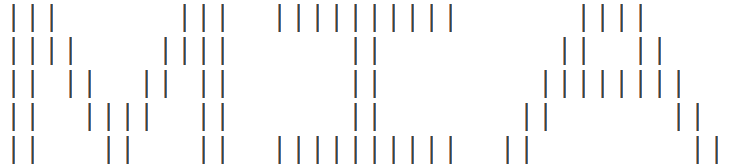
\includegraphics[scale=0.5]{./images/man_cover.png} \vspace{.5cm} \\ Project Name \\  Manual \& Programming Documentation}
\author{Developer: Antonius Torode \\ Affiliation \\ Department}
\date{Version -- \Version \\ Latest update: \today}

\makeindex
%\addcontentsline{toc}{chapter}{Index}
%END_FOLD

%%% Document Starts now
\begin{document}

%Begin the front matter. Front matter pages are numbered with roman numerals.
\frontmatter
%Begins title page.
\maketitle
\thispagestyle{empty}
\pagestyle{empty}

%Copyright page.
\pagestyle{empty}
%% copyrightpage
\begingroup
\footnotesize
\parindent 0pt
\parskip \baselineskip
\textcopyright{} 2026 Antonius Torode \\
All rights reserved.

This work may be distributed and/or modified under the conditions of Antonius' General Purpose License (AGPL).

The Original Maintainer of this work is: Antonius Torode.

The Current Maintainer of this work is: Antonius Torode.

This document is designed for the sole purpose of providing a template for writing a manual/book in LaTeX.

Hosted at: \url{https://github.com/torodean}

\begin{center}
\begin{tabular}{ll}
This document is continuously under development. \\
Most Current Revision Date (Version \Version): &  \today
\end{tabular}
\end{center}

\vfill

Torode, A.\\
\hspace*{2em} Project Name Manual. \\
\hspace*{2em} Affiliation -- \\
\hspace*{2em} Department. \\
\hspace*{2em} 2026. \\
\hspace*{2em} Version: \Version \\

\endgroup
\clearpage


%Begins table of contents
\tableofcontents

%Begins blank page.
\newpage
\vspace*{\fill}
\begin{center}
	\textit{This page intentionally left blank. \\ (Yes, this is a contradiction.)}
\end{center}
\vspace*{\fill}

%Begin the mainmatter. Main matter pages are numbered with arabic numerals.
\setlength{\parindent}{0pt}
\mainmatter
\pagestyle{fancy}

\newpage
% This chapter demonstrates every formatting option the template provides.
% Each demo shows the LaTeX source first, then the rendered result, so new
% users can copy the source directly. Delete this file's body (or the whole
% chapter) once real content replaces it. Keep each demo in sync with
% TeX_files/definitions.tex and TeX_files/settings.tex.
\chapter{Template Usage}
\thispagestyle{fancy}
\label{chapter:template}

This chapter explains how to add content to the manual and demonstrates every custom formatting option. Each demo shows the LaTeX source first, then the rendered result, so you can copy the source and adapt it.

\section{Adding a Chapter}

Each chapter lives in its own file under \texttt{TeX\_files/}. To add one:

\begin{enumerate}
	\item Create \texttt{TeX\_files/<name>.tex}.
	\item Begin the file with a chapter heading and label, as shown below.
	\item Add an \lstinline|\include| line for it in \texttt{Manual.tex}, wrapped in \lstinline|\newpage|.
\end{enumerate}

\begin{lstlisting}[style=latexstyle]
% TeX_files/Example.tex
\chapter{Example Chapter}
\thispagestyle{fancy}
\label{chapter:example}

% Body text goes here.
\end{lstlisting}

\begin{lstlisting}[style=latexstyle]
% In Manual.tex, add the chapter after the last one:
\newpage
\include{./TeX_files/Example}
\end{lstlisting}

\section{Text Formatting}

\subsection{Emphasis and Fonts}

\begin{lstlisting}[style=latexstyle]
\textbf{Bold text}, \textit{italic text}, \texttt{monospace text},
\textsc{small caps}, \underline{underlined text}.
\end{lstlisting}

\textbf{Bold text}, \textit{italic text}, \texttt{monospace text}, \textsc{small caps}, \underline{underlined text}.

\subsection{Sections}

Chapters are divided with \lstinline|\section|, \lstinline|\subsection|, and \lstinline|\subsubsection|. They are numbered automatically and appear in the table of contents.

\begin{lstlisting}[style=latexstyle]
\section{A Top Level Heading}
\subsection{A Second Level Heading}
\subsubsection{A Third Level Heading}
\end{lstlisting}

\subsection{Lists}

\begin{lstlisting}[style=latexstyle]
\begin{itemize}
	\item An itemize bullet.
	\item A second bullet.
\end{itemize}

\begin{enumerate}
	\item An enumerated item.
	\item A second item.
\end{enumerate}
\end{lstlisting}

\begin{itemize}
	\item An itemize bullet.
	\item A second bullet.
\end{itemize}

\begin{enumerate}
	\item An enumerated item.
	\item A second item.
\end{enumerate}

\subsection{Tables}

\begin{lstlisting}[style=latexstyle]
\begin{center}
	\begin{tabular}{l|l|l}
		Column one & Column two & Column three \\
		\hline
		cell & cell & cell \\
		cell & cell & cell \\
	\end{tabular}
\end{center}
\end{lstlisting}

\begin{center}
	\begin{tabular}{l|l|l}
		Column one & Column two & Column three \\
		\hline
		cell & cell & cell \\
		cell & cell & cell \\
	\end{tabular}
\end{center}

The \texttt{\{l|l|l\}} argument gives one left-aligned column per letter, with vertical rules between them. Use \texttt{|} where you want a line and \texttt{c} or \texttt{r} for centered or right-aligned columns.

\subsection{Cross References, Footnotes, and URLs}

Label anything you need to reference with \lstinline|\label{unique_name}|, then point at it with \lstinline|\ref{...}|. Label names use underscores, not dashes. Labels always go on the environment or sectioning command they name.

\begin{lstlisting}[style=latexstyle]
A cross reference to the first theorem: \ref{thm:example}.
A footnote\footnote{Footnotes render at the bottom of the page.}.
A URL: \url{https://github.com/torodean}
\end{lstlisting}

A cross reference to the first theorem: \ref{thm:example}. A footnote\footnote{Footnotes render at the bottom of the page.}. A URL: \url{https://github.com/torodean}

\subsection{Index Terms}

The \lstinline|\idx{term}| command prints a term in bold and adds it to the back-of-book index. Use it for key concepts a reader would search for. Plain \lstinline|\index{term}| adds an unbolded index entry without printing anything extra.

\begin{lstlisting}[style=latexstyle]
The \idx{template} prints bold and indexes the term.
This sentence mentions the \index{indexing} without bolding it.
\end{lstlisting}

The \idx{template} prints bold and indexes the term.
This sentence mentions the \index{indexing} without bolding it.

\subsection{Math}

Inline math goes between dollar signs; display math goes in an equation environment.

\begin{lstlisting}[style=latexstyle]
Inline math ($a^2 + b^2 = c^2$) and display math:

\begin{equation}
	e^{i\pi} + 1 = 0
\end{equation}
\end{lstlisting}

Inline math ($a^2 + b^2 = c^2$) and display math:

\begin{equation}
	e^{i\pi} + 1 = 0
\end{equation}

\section{Code Listings}

Code goes in a \texttt{lstlisting} environment. The \texttt{style=} option picks one of the language styles defined in \texttt{settings.tex}. The styles available are \texttt{terminalstyle}, \texttt{shellstyle}, \texttt{cppstyle}, \texttt{cmakestyle}, \texttt{gitstyle}, \texttt{makestyle}, \texttt{pythonstyle}, and \texttt{latexstyle}. Use \texttt{terminalstyle} for interactive sessions and \texttt{shellstyle} for scripts.

\begin{latexsource}
\begin{lstlisting}[style=cppstyle]
int add(int a, int b)
{
	return a + b;  // Return the sum of a and b.
}
\end{lstlisting}
\end{latexsource}

Which renders as:

\begin{lstlisting}[style=cppstyle]
int add(int a, int b)
{
	return a + b;  // Return the sum of a and b.
}
\end{lstlisting}

For a single short snippet inside a sentence, use the lstinline command. It takes any character you like as the delimiter, as in \texttt{\string\lstinline|code|}.

The \texttt{latexsource} environment is a \texttt{lstlisting} block with the \texttt{latexstyle} under a different name. Use it whenever the source you are showing contains a \texttt{lstlisting} environment itself; a normal \texttt{lstlisting} block would end at the inner \lstinline|\end{lstlisting}|.

\subsection{terminalstyle}

\begin{lstlisting}[style=terminalstyle]
$ cd ~/git/Antonius-Templates
$ pdflatex Manual.tex      # compile the manual
\end{lstlisting}

\subsection{shellstyle}

\begin{lstlisting}[style=shellstyle]
#!/bin/bash
# A comment in a shell script.
echo "Hello, World!"
\end{lstlisting}

\subsection{pythonstyle}

\begin{lstlisting}[style=pythonstyle]
def add(a, b):
    return a + b
\end{lstlisting}

\subsection{cmakestyle}

\begin{lstlisting}[style=cmakestyle]
cmake_minimum_required(VERSION 3.10)
project(example CXX)
add_executable(example main.cpp)
\end{lstlisting}

\subsection{gitstyle}

\begin{lstlisting}[style=gitstyle]
git commit -m "A commit message."
\end{lstlisting}

\subsection{makestyle}

\begin{lstlisting}[style=makestyle]
all: Manual.pdf

Manual.pdf: Manual.tex
	pdflatex Manual.tex
\end{lstlisting}

\section{Callout Boxes}

The boxed environments below are defined in \texttt{TeX\_files/definitions.tex}. The mdframed boxes each take an optional title in square brackets and a label in curly braces; the label argument is required, even when you never reference the box, so pass empty curly braces if you do not need one. The tcolorbox boxes take no arguments.

\subsection{Fancy Box (mdframed)}

The general purpose numbered box. Use it for callouts that do not fit a more specific environment.

\begin{lstlisting}[style=latexstyle]
\begin{fancybox}[Title]{label:name}
	Box content goes here.
\end{fancybox}
\end{lstlisting}

\begin{fancybox}[Fancy Box]{fancy_box_example}
	The fancybox is a general purpose orange box. Leave the label empty (\lstinline|\begin{fancybox}[Title]{}|) when the box does not need to be referenced.
\end{fancybox}

\subsection{Theorem, Lemma, Proof, and Definition (mdframed)}

Numbered blue, green, and red boxes for formal statements, plus a gray definition box. Each takes an optional title and an optional label.

\begin{lstlisting}[style=latexstyle]
\begin{theo}[Theorem Title]{thm:label}
	Theorem content.
\end{theo}

\begin{lemm}[Lemma Title]{lem:label}
	Lemma content.
\end{lemm}

\begin{prf}[Proof Title]{prf:label}
	Proof content, ends with a QED symbol.
\end{prf}

\begin{defn}[Definition Title]{def:label}
	Definition content.
\end{defn}
\end{lstlisting}

\begin{theo}[Theorem Title]{thm:example}
	The theo environment renders a blue numbered theorem box. Referenced here as \ref{thm:example}.
\end{theo}

\begin{lemm}[Lemma Title]{lem:example}
	The lemm environment renders a green numbered lemma box. Referenced here as \ref{lem:example}.
\end{lemm}

\begin{prf}[Proof Title]{prf:example}
	The prf environment renders a red numbered proof box and ends with a QED symbol.
\end{prf}

\begin{defn}[Definition Title]{def:example}
	The defn environment renders a gray numbered definition box.
\end{defn}

\subsection{Questions (tcolorbox)}

An orange box for open questions about a section. Write plain item lines; the environment wraps them in a list for you.

\begin{lstlisting}[style=latexstyle]
\begin{questions}
	\item First question.
	\item Second question.
\end{questions}
\end{lstlisting}

\begin{questions}
	\item The questions environment is an orange box that wraps an itemize list.
	\item Use it to collect open questions about a section.
\end{questions}

\subsection{Interesting Note, Quotation, and URL (tcolorbox)}

\begin{lstlisting}[style=latexstyle]
\begin{interestingnote}
	Trivia or an aside.
\end{interestingnote}

\begin{quotationbox}
	A quotation.
\end{quotationbox}

\begin{urlbox}
	A link: \url{https://github.com/torodean}
\end{urlbox}
\end{lstlisting}

\begin{interestingnote}
	The interestingnote environment is a green box with a lightbulb icon. Use it for trivia or asides that are not essential.
\end{interestingnote}

\begin{quotationbox}
	The quotationbox environment is a purple box with a quote icon.
\end{quotationbox}

\begin{urlbox}
	The urlbox environment is a blue box for references. Example: \url{https://github.com/torodean}
\end{urlbox}

\subsection{Unfinished Banner}

Place \lstinline|\unfinished| on its own line to mark a section as incomplete. It renders the banner below.

\begin{lstlisting}[style=latexstyle]
\unfinished
\end{lstlisting}

The command renders this banner:

\vspace{10pt}
\unfinished


\newpage
%Add new chapters here, each wrapped in \newpage.
%\include{./TeX_files/ChapterName}

%Begin the backmatter.
\backmatter
% Appendices. Each \chapter inside this environment is lettered (A, B, C, ...)
% instead of numbered. Add \section content below as usual.
\begin{appendices}
	\chapter{Appendix A}

	% Appendix content goes here.

\end{appendices}


{\footnotesize
\begin{thebibliography}{99}
	\bibitem{example} [TODO: References.]
\end{thebibliography}
}

\printindex

\end{document}
